\documentclass[oneside, 11pt]{article}

\usepackage[T1]{fontenc}
\usepackage[utf8]{inputenc}
\usepackage[dutch]{babel}

\usepackage{fouriernc}
\usepackage[detect-all, load-configurations=binary,
            separate-uncertainty=true, per-mode=symbol,
            retain-explicit-plus, range-phrase={ tot }]{siunitx}

\usepackage{setspace}
\setstretch{1.2}

\setlength{\parskip}{\smallskipamount}
\setlength{\parindent}{0pt}

\usepackage{geometry}
\geometry{marginparwidth=0.5cm, verbose, a4paper, tmargin=3cm, bmargin=3cm, lmargin=2cm, rmargin=2cm}

\usepackage{float}

\usepackage[fleqn]{amsmath}
\numberwithin{equation}{section}
\numberwithin{figure}{section}

\usepackage{graphicx}
\graphicspath{{Figures/}}
\usepackage{subfig}

\usepackage{tikz}
\usetikzlibrary{plotmarks}

\usepackage{fancyhdr}
\pagestyle{fancy}
\fancyhf{}
\rhead{\thepage}
\renewcommand{\footrulewidth}{0pt}
\renewcommand{\headrulewidth}{0pt}

\usepackage{relsize}
\usepackage{xspace}
\usepackage{url}

\newcommand{\figref}[1]{Figuur~\ref{#1}}

\newcommand{\hisparc}{\textsmaller{HiSPARC}\xspace}
\newcommand{\kascade}{\textsmaller{KASCADE}\xspace}
\newcommand{\sapphire}{\textsmaller{SAPPHiRE}\xspace}
\newcommand{\jsparc}{\textsmaller{jSparc}\xspace}
\newcommand{\hdf}{\textsmaller{HDF5}\xspace}
\newcommand{\aires}{\textsmaller{AIRES}\xspace}
\newcommand{\csv}{\textsmaller{CSV}\xspace}
\newcommand{\python}{\textsmaller{PYTHON}\xspace}
\newcommand{\corsika}{\textsmaller{CORSIKA}\xspace}
\newcommand{\labview}{\textsmaller{LabVIEW}\xspace}
\newcommand{\daq}{\textsmaller{DAQ}\xspace}
\newcommand{\adc}{\textsmaller{ADC}\xspace}
\newcommand{\adcs}{\textsmaller{ADC}s\xspace}
\newcommand{\Adcs}{A\textsmaller{DC}s\xspace}
\newcommand{\hi}{\textsc{h i}\xspace}
\newcommand{\hii}{\textsc{h ii}\xspace}
\newcommand{\mip}{\textsmaller{MIP}\xspace}
\newcommand{\hisparcii}{\textsmaller{HiSPARC II}\xspace}
\newcommand{\hisparciii}{\textsmaller{HiSPARC III}\xspace}
\newcommand{\pmt}{\textsmaller{PMT}\xspace}
\newcommand{\pmts}{\textsmaller{PMT}s\xspace}

\DeclareSIUnit{\electronvolt}{\ensuremath{\mathrm{e\!\!\:V}}}

\DeclareSIUnit{\unitsigma}{\ensuremath{\sigma}}
\DeclareSIUnit{\mip}{\textsmaller{MIP}}
\DeclareSIUnit{\adc}{\textsmaller{ADC}}

\DeclareSIUnit{\gauss}{G}
\DeclareSIUnit{\parsec}{pc}
\DeclareSIUnit{\year}{yr}




\title{Uitlijnen van de \adcs}
\author{D. B. R. A. Fokkema}
\doctheorie{2}{UA}
\version{1.0}


\begin{document}

\maketitle

\section{De \hisparc uitleeselektronica}

De \hisparc detectoren bestaan uit een rechthoekige \emph{scintillator}
die via een driehoekige \emph{lichtgeleider} verbonden zijn met een
\emph{fotobuis} (\pmt \footnote{\pmt staat voor PhotoMultiplier Tube
(fotoversterkerbuis).}).  De fotobuis is verantwoordelijk voor de detectie
van de kleine lichtflitsjes in de scintillator die worden veroorzaakt door
geladen deeltjes uit de kosmische straling.  Deze lichtflitsjes worden
omgezet in een kleine elektrische stroom.  Deze stroom wordt door een
bekende weerstand geleid en de spanning over deze weerstand kan worden
gemeten.  Hoe feller het lichtflitsje, hoe hoger de spanning
(\figref{fig:schema-pmt}).

\begin{figure}
\centering
\documentclass{article}

\usepackage{tikz}
\usetikzlibrary{circuits.ee.IEC}

%\tikzset{circuit declare symbol=terminal}
%\tikzset{set terminal graphic={draw, generic circle IEC, minimum size=4pt}}
\tikzset{circuit declare symbol=voltmeter}
\tikzset{set voltmeter graphic={draw, generic circle IEC, minimum size=6mm, info=center:V}}

\begin{document}

\begin{tikzpicture}[x=2cm,y=2cm,circuit ee IEC]
\draw (0, -.2) node[ground,point down] {} -- (0, 0) to[resistor={info=R}] (0, 1) -- (1, 1) to[voltmeter={info=right:ADC}] (1, 0) -- (0, 0);

\draw (-1, -.2) node[ground,point down] {} -- (-1, 0) to[battery={volt={\approx 900}}] (-1, 2) -- (0, 2) to[resistor={info={PMT}}] (0, 1);
\end{tikzpicture}

\end{document}
\caption{Vereenvoudigd elektrisch schema van het uitlezen van een PMT.  Op
de PMT staat een hoogspanning van ongeveer \SI{900}{\volt}, variërend van
buis tot buis.  De stroom uit de PMT wordt via een bekende weerstand $R$
naar de aarde geleid.  De spanning over deze weerstand wordt uitgelezen
door de \adcs.}
\label{fig:schema-pmt}
\end{figure}

De \pmts zijn via lange kabels verbonden met de uitleeselektronica van
\hisparc (het `rode kastje').  De uitleeselektronica is verantwoordelijk
voor het omzetten van de elektrische spanningen van de \pmts in een
signaal dat de computer kan begrijpen.

Iedere \SI{2.5}{\nano\second} wordt het signaal gemeten met een
nauwkeurigheid van \num{4096} stapjes tussen ongeveer
\SIrange{+0.113}{-2}{\volt}, afhankelijk van de elektronica.  Deze stapjes
noemen we \emph{\adc counts}.  Het \emph{analoge} signaal wordt zo omgezet
in een \emph{digitaal} signaal.  De chip die daarvoor verantwoordelijk is
heet dan ook een \emph{Analog Digital Converter} (\adc).  Snelle \adcs
zijn echter erg duur.  Daarom is ervoor gekozen om niet één \adc te
gebruiken die samplet met \SI{2.5}{\nano\second}, maar twéé \adcs die
ieder samplen met \SI{5}{\nano\second}.  Deze twee \adcs worden dan om en
om gebruikt.  Een digitale klok met een frequentie van
\SI{200}{\mega\hertz} regelt het uitlezen.  Eén \adc wordt uitgelezen als
de klokpuls omhoog gaat, de ander als de klokpuls omlaag gaat.  Zie
\figref{fig:ADC-sampling} voor een schematische voorstelling.

\begin{figure}
\centering
\documentclass{standalone}

\usepackage{tikz}
\usetikzlibrary{plotmarks}

\begin{document}

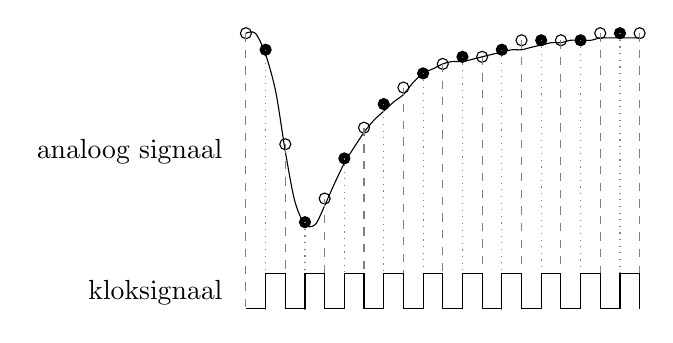
\begin{tikzpicture}[y=3cm]
\draw[smooth] plot coordinates {(0.00, -0.00) (0.12, -0.00) (0.25, -0.09) (0.38, -0.25) (0.50, -0.50) (0.62, -0.71) (0.75, -0.81) (0.88, -0.81) (1.00, -0.73) (1.12, -0.64) (1.25, -0.55) (1.38, -0.48) (1.50, -0.42) (1.62, -0.37) (1.75, -0.33) (1.88, -0.29) (2.00, -0.26) (2.12, -0.21) (2.25, -0.17) (2.38, -0.15) (2.50, -0.13) (2.62, -0.12) (2.75, -0.12) (2.88, -0.11) (3.00, -0.10) (3.12, -0.09) (3.25, -0.08) (3.38, -0.07) (3.50, -0.07) (3.62, -0.06) (3.75, -0.05) (3.88, -0.04) (4.00, -0.04) (4.12, -0.03) (4.25, -0.03) (4.38, -0.03) (4.50, -0.02) (4.62, -0.02) (4.75, -0.02) (4.88, -0.02) (5.00, -0.02)};
\draw[mark=o, only marks] plot coordinates {(0.00, 0.00) (0.50, -0.47) (1.00, -0.70) (1.50, -0.40) (2.00, -0.23) (2.50, -0.13) (3.00, -0.10) (3.50, -0.03) (4.00, -0.03) (4.50, 0.00) (5.00, 0.00)};
\draw[mark=*, only marks] plot coordinates {(0.25, -0.07) (0.75, -0.80) (1.25, -0.53) (1.75, -0.30) (2.25, -0.17) (2.75, -0.10) (3.25, -0.07) (3.75, -0.03) (4.25, -0.03) (4.75, 0.00)};

\draw[gray,dashed] (0.00, 0.00) -- (0.00, -3.5cm);
\draw[gray,dashed] (0.50, -0.47) -- (0.50, -3.5cm);
\draw[gray,dashed] (1.00, -0.70) -- (1.00, -3.5cm);
\draw[gray,dashed] (1.50, -0.40) -- (1.50, -3.5cm);
\draw[gray,dashed] (2.00, -0.23) -- (2.00, -3.5cm);
\draw[gray,dashed] (2.50, -0.13) -- (2.50, -3.5cm);
\draw[gray,dashed] (3.00, -0.10) -- (3.00, -3.5cm);
\draw[gray,dashed] (3.50, -0.03) -- (3.50, -3.5cm);
\draw[gray,dashed] (4.00, -0.03) -- (4.00, -3.5cm);
\draw[gray,dashed] (4.50, 0.00) -- (4.50, -3.5cm);
\draw[gray,dashed] (5.00, 0.00) -- (5.00, -3.5cm);

\draw[gray,dotted] (0.25, -0.07) -- (0.25, -3.5cm);
\draw[gray,dotted] (0.75, -0.80) -- (0.75, -3.5cm);
\draw[gray,dotted] (1.25, -0.53) -- (1.25, -3.5cm);
\draw[gray,dotted] (1.75, -0.30) -- (1.75, -3.5cm);
\draw[gray,dotted] (2.25, -0.17) -- (2.25, -3.5cm);
\draw[gray,dotted] (2.75, -0.10) -- (2.75, -3.5cm);
\draw[gray,dotted] (3.25, -0.07) -- (3.25, -3.5cm);
\draw[gray,dotted] (3.75, -0.03) -- (3.75, -3.5cm);
\draw[gray,dotted] (4.25, -0.03) -- (4.25, -3.5cm);
\draw[gray,dotted] (4.75, 0.00) -- (4.75, -3.5cm);

\draw[const plot,yshift=-3.5cm,yscale=.15] plot coordinates {(0.00, 0.00) (0.25, 1.00) (0.50, 0.00) (0.75, 1.00) (1.00, 0.00) (1.25, 1.00) (1.50, 0.00) (1.75, 1.00) (2.00, 0.00) (2.25, 1.00) (2.50, 0.00) (2.75, 1.00) (3.00, 0.00) (3.25, 1.00) (3.50, 0.00) (3.75, 1.00) (4.00, 0.00) (4.25, 1.00) (4.50, 0.00) (4.75, 1.00) (5.00, 0.00)};

\node[left=5pt] at (0, -3.3cm) {kloksignaal};
\node[left=5pt] at (0, -1.5cm) {analoog signaal};

\end{tikzpicture}

\end{document}
\caption{Het samplen van het analoge signaal wordt uitgevoerd door twee
\adcs.  De \adcs nemen om de beurt een sample en zetten het analoge
signaal om in een digitaal signaal.  Omdat het digitale signaal slechts
\num{4096} stapjes heeft, is het een \emph{benadering} van het analoge
signaal.  Dit kun je zien aan de samples die niet exact op het analoge
signaal liggen.  Eén van de \adcs (witte rondjes) wordt geklokt op de
neergaande flank van het kloksignaal, de andere \adc (zwarte rondjes)
wordt geklokt op de opgaande flank.}
\label{fig:ADC-sampling}
\end{figure}

Het is belangrijk dat de twee \adcs zijn \emph{uitgelijnd}.  Dat wil
zeggen: dat de \adcs het eens zijn over hoeveel \adc counts overeenkomen
met, bijvoorbeeld, \SI{1}{\volt}.  Zijn de \adcs ten opzichte van elkaar
verschoven, dan ontstaat een driehoekig digitaal signaal zoals weergegeven
in \figref{fig:unaligned-adcs}.

\begin{figure}
\centering
\documentclass{standalone}

\usepackage{tikz}
\usetikzlibrary{plotmarks}
\usepackage{siunitx}

\begin{document}

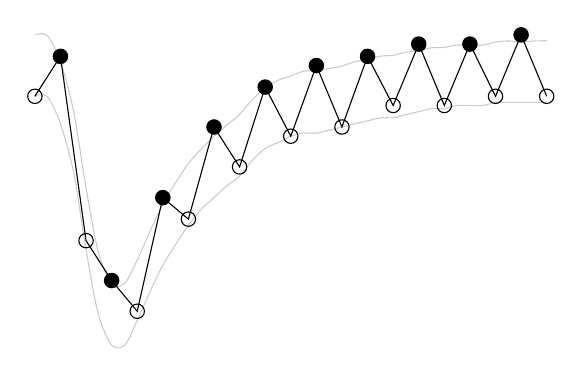
\begin{tikzpicture}[scale=1.3,y=3cm]
\draw[smooth,black!20] plot coordinates {(0.00, -0.00) (0.12, -0.00) (0.25, -0.09) (0.38, -0.25) (0.50, -0.50) (0.62, -0.71) (0.75, -0.81) (0.88, -0.81) (1.00, -0.73) (1.12, -0.64) (1.25, -0.55) (1.38, -0.48) (1.50, -0.42) (1.62, -0.37) (1.75, -0.33) (1.88, -0.29) (2.00, -0.26) (2.12, -0.21) (2.25, -0.17) (2.38, -0.15) (2.50, -0.13) (2.62, -0.12) (2.75, -0.12) (2.88, -0.11) (3.00, -0.10) (3.12, -0.09) (3.25, -0.08) (3.38, -0.07) (3.50, -0.07) (3.62, -0.06) (3.75, -0.05) (3.88, -0.04) (4.00, -0.04) (4.12, -0.03) (4.25, -0.03) (4.38, -0.03) (4.50, -0.02) (4.62, -0.02) (4.75, -0.02) (4.88, -0.02) (5.00, -0.02)};

\draw[smooth,black!20] plot coordinates {(0.00, 0.2000) (0.12, 0.1981) (0.25, 0.1126) (0.38, -0.0517) (0.50, -0.2986) (0.62, -0.5075) (0.75, -0.6120) (0.88, -0.6082) (1.00, -0.5331) (1.12, -0.4439) (1.25, -0.3508) (1.38, -0.2786) (1.50, -0.2188) (1.62, -0.1732) (1.75, -0.1305) (1.88, -0.0925) (2.00, -0.0593) (2.12, -0.0127) (2.25, 0.0272) (2.38, 0.0528) (2.50, 0.0661) (2.62, 0.0813) (2.75, 0.0832) (2.88, 0.0908) (3.00, 0.0984) (3.12, 0.1126) (3.25, 0.1202) (3.38, 0.1307) (3.50, 0.1335) (3.62, 0.1430) (3.75, 0.1478) (3.88, 0.1582) (4.00, 0.1592) (4.12, 0.1668) (4.25, 0.1658) (4.38, 0.1668) (4.50, 0.1763) (4.62, 0.1801) (4.75, 0.1772) (4.88, 0.1801) (5.00, 0.1810)};

\draw[mark=o, only marks] plot coordinates {(0.00, 0.00) (0.50, -0.47) (1.00, -0.70) (1.50, -0.40) (2.00, -0.23) (2.50, -0.13) (3.00, -0.10) (3.50, -0.03) (4.00, -0.03) (4.50, 0.00) (5.00, 0.00)};

\draw[mark=*, only marks] plot coordinates {(0.25, 0.13) (0.75, -0.60) (1.25, -0.33) (1.75, -0.10) (2.25, 0.03) (2.75, 0.10) (3.25, 0.13) (3.75, 0.17) (4.25, 0.17) (4.75, 0.20)};

\draw plot coordinates {(0.00, 0.00) (0.25, 0.13) (0.50, -0.47) (0.75, -0.60) (1.00, -0.70) (1.25, -0.33) (1.50, -0.40) (1.75, -0.10) (2.00, -0.23) (2.25, 0.03) (2.50, -0.13) (2.75, 0.10) (3.00, -0.10) (3.25, 0.13) (3.50, -0.03) (3.75, 0.17) (4.00, -0.03) (4.25, 0.17) (4.50, 0.00) (4.75, 0.20) (5.00, 0.00)};

\end{tikzpicture}

\end{document}
\caption{Wanneer de twee \adcs niet netjes zijn uitgelijnd, zien ze het
analoge signaal met een verschuiving.  Hoewel iedere \adc het signaal
netjes samplet, ziet de combinatie van de twee \adcs er slecht uit.}
\label{fig:unaligned-adcs}
\end{figure}


\section{Uitlijnen van de \adcs}

Het uitlijnen van de \adcs is een volautomatisch proces, maar moet wel
door de gebruiker gestart worden.  Doorloop daarvoor het volgende
stappenplan:
\begin{enumerate}
\item Zorg er voor dat het data acquisitie programma (\daq) draait.
\item Stop de data acquisitie door op de knop \emph{STOP DAQ} te klikken
(\figref{fig:stop-daq}).
\item Als daarom gevraagd wordt, kies \emph{Expert Mode}
(\figref{fig:expert-mode}).
\item Als het programma weer draait, klik dan op de tab \emph{ADC
alignment}, rechtsboven in beeld (\figref{fig:alignment-tab}).
\item Klik op de \emph{Start Alignment} knop, rechtsboven
(\figref{fig:start-alignment}).
\item Nadat de procedure is afgerond, kies \emph{Yes} op de vraag:
\emph{Do you want to save current (alignment) settings?}
(\figref{fig:save-alignment-settings}).
\item Klik op de knop \emph{DAQ MODE} (\figref{fig:start-daq}).
\end{enumerate}

\begin{figure}
\centering
\subfloat[]{
\includegraphics[width=.3\linewidth]{stop-daq}
  \label{fig:stop-daq}}
\hfill
\subfloat[]{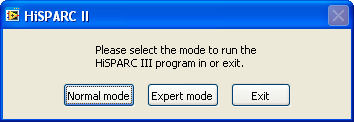
\includegraphics[width=.3\linewidth]{expert-mode}
  \label{fig:expert-mode}}
\hfill
\subfloat[]{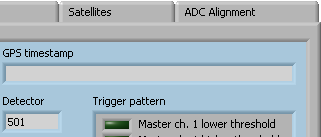
\includegraphics[width=.3\linewidth]{alignment-tab}
  \label{fig:alignment-tab}}

\vspace{1em}

\subfloat[]{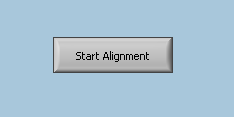
\includegraphics[width=.3\linewidth]{start-alignment}
  \label{fig:start-alignment}}
\hfill
\subfloat[]{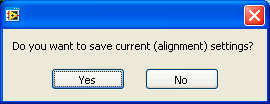
\includegraphics[width=.3\linewidth]{save-alignment-settings}
  \label{fig:save-alignment-settings}}
\hfill
\subfloat[]{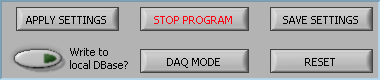
\includegraphics[width=.3\linewidth]{start-daq}
  \label{fig:start-daq}}
\caption{Screenshots van de \daq software.  Deze verduidelijken de
verschillende stappen voor het uitlijnen van de \adcs.  Zie de
beschrijving in de lopende tekst.}
\end{figure}

Voor meer informatie over de bediening van de \daq software, zie
\cite{software-handleiding}.


\begin{thebibliography}{9}
\bibitem{software-handleiding} Het \hisparc team, \emph{\hisparc software
documentatie} (2009--2012),
\url{http://docs.hisparc.nl/station-software/doc/}.
\end{thebibliography}

\end{document}
